% THIS IS SIGPROC-SP.TEX - VERSION 3.1
% WORKS WITH V3.2SP OF ACM_PROC_ARTICLE-SP.CLS
% APRIL 2009
%
% It is an example file showing how to use the 'acm_proc_article-sp.cls' V3.2SP
% LaTeX2e document class file for Conference Proceedings submissions.
% ----------------------------------------------------------------------------------------------------------------
% This .tex file (and associated .cls V3.2SP) *DOES NOT* produce:
%       1) The Permission Statement
%       2) The Conference (location) Info information
%       3) The Copyright Line with ACM data
%       4) Page numbering
% ---------------------------------------------------------------------------------------------------------------
% It is an example which *does* use the .bib file (from which the .bbl file
% is produced).
% REMEMBER HOWEVER: After having produced the .bbl file,
% and prior to final submission,
% you need to 'insert'  your .bbl file into your source .tex file so as to provide
% ONE 'self-contained' source file.
%
% Questions regarding SIGS should be sent to
% Adrienne Griscti ---> griscti@acm.org
%
% Questions/suggestions regarding the guidelines, .tex and .cls files, etc. to
% Gerald Murray ---> murray@hq.acm.org
%
% For tracking purposes - this is V3.1SP - APRIL 2009

\documentclass{acm_proc_article-sp}

\usepackage{graphicx}
\usepackage{subcaption} 
\usepackage{dsfont}
\usepackage{braket}
\usepackage{hyperref}
\usepackage{multirow}

\usepackage{amsmath}
\usepackage{amssymb}
\usepackage{braket}
\usepackage{xcolor}

\usepackage{pgfplots}
\usepackage{algorithm}
\usepackage{listings, listings-rust}

\begin{document}

\pagenumbering{arabic}

\title{Safety e Security del Codice}
\subtitle{Incidenti e Soluzioni}
%
% You need the command \numberofauthors to handle the 'placement
% and alignment' of the authors beneath the title.
%
% For aesthetic reasons, we recommend 'three authors at a time'
% i.e. three 'name/affiliation blocks' be placed beneath the title.
%
% NOTE: You are NOT restricted in how many 'rows' of
% "name/affiliations" may appear. We just ask that you restrict
% the number of 'columns' to three.
%
% Because of the available 'opening page real-estate'
% we ask you to refrain from putting more than six authors
% (two rows with three columns) beneath the article title.
% More than six makes the first-page appear very cluttered indeed.
%
% Use the \alignauthor commands to handle the names
% and affiliations for an 'aesthetic maximum' of six authors.
% Add names, affiliations, addresses for
% the seventh etc. author(s) as the argument for the
% \additionalauthors command.
% These 'additional authors' will be output/set for you
% without further effort on your part as the last section in
% the body of your article BEFORE References or any Appendices.

\numberofauthors{1} %  in this sample file, there are a *total*
% of EIGHT authors. SIX appear on the 'first-page' (for formatting
% reasons) and the remaining two appear in the \additionalauthors section.
%
\author{
% You can go ahead and credit any number of authors here,
% e.g. one 'row of three' or two rows (consisting of one row of three
% and a second row of one, two or three).
%
% The command \alignauthor (no curly braces needed) should
% precede each author name, affiliation/snail-mail address and
% e-mail address. Additionally, tag each line of
% affiliation/address with \affaddr, and tag the
% e-mail address with \email.
%
% 1st. author
\alignauthor
Francesco Bernini\\
       \affaddr{Università di Parma}\\
}
% There's nothing stopping you putting the seventh, eighth, etc.
% author on the opening page (as the 'third row') but we ask,
% for aesthetic reasons that you place these 'additional authors'
% in the \additional authors block, viz.

\maketitle
\begin{abstract}
This paper explains how the Grover algorithm is structured and how it solves the unstructured search problem. There will be different visualization and explanations for each step of the algorithm and the circuits needed to build a quantum system solving the Grover algorithm. Furthermore the paper will analyze the behavior of the algorithm on different scenarios and will give different techniques to improve the solution.
\end{abstract}

\section{Introduzione}
Negli ultimi anni, la sicurezza informatica è diventata una priorità per aziende, governi e sviluppatori, complice la crescente sofisticatezza degli attacchi e delle vulnerabilità software. La maggior parte di questi problemi origina da una erronea gestione della memoria \cite{MemoryProblems}, ma anche un'imprecisa gestione della concorrenza, un errata configurazione di sistemi o errori logici di programmazione possono portare a malfunzionamenti.


Il software è ormai parte integrante di quasi tutte le attività umane ed alcune di esse possono descriversi come ``safety-critical'', ovvero dove la sicurezza del corretto funzionamento del codice (anche in caso di situazioni eccezionali) deve essere garantita. Tra queste attività troviamo sicuramente tutte quelle che coinvolgono l'ambito avionico, automotive, biomedicale perché possono avere ripercussioni dirette sulla salute. Per lo sviluppo di questa tipologia di programmi vi sono linguaggi, tecniche di programmazione e software di supporto ad-hoc.


Ovviamente non tutti i tipi di software hanno questi requisiti stringenti di correttezza, come quelli relativi al mondo videoludico o al mondo della Data Science, per citarne alcuni. Tuttavia errori in entrambe queste categorie possono portare ad ingenti perdite di denaro, per motivi diversi \cite{NintendoLooseMoney} \cite{LondonWhale}. 


In generale non è sempre possibile scegliere un linguaggio di programmazione che offre funzionalità volte alla gestione della memoria automatica come il \textit{garbage collector} perché esso richiede risorse computazionali che in certi ambiti non sono disponibili e inoltre rende impossibile determinare il tempo entro il quale certe operazioni verranno effettuate (requisito fondamentale dei sistemi real-time). Sono comunque disponibili diverse soluzioni che verranno trattate in questo documento.

%sia in applicazioni più generali, come browser, sistemi operativi e infrastrutture cloud.

%Nei sistemi safety-critical, dove il software deve rispettare requisiti stringenti di affidabilità e prevedibilità, l’uso di linguaggi con garbage collector è spesso sconsigliato per via dell’imprevedibilità nella gestione della memoria. Tuttavia, anche nei sistemi non safety-critical, l’assenza di protezioni integrate nei linguaggi tradizionali come C e C++ rende il codice vulnerabile a exploit come buffer overflow e use-after-free, ampiamente sfruttati per eseguire codice malevolo o compromettere l’integrità dei dati. Inoltre, molti linguaggi non offrono strumenti efficaci per gestire la concorrenza, esponendo il software a problemi come race conditions e deadlock.

%Per affrontare queste criticità esistono diverse soluzioni. Una strategia diffusa è l’adozione di analizzatori statici, strumenti che aiutano a individuare vulnerabilità nel codice scritto in linguaggi memory-unsafe. Un’altra possibilità è l’uso di sottoinsiemi sicuri di linguaggi tradizionali, che limitano l’uso di funzionalità pericolose mantenendo la compatibilità con il codice esistente. Infine, la soluzione più radicale è l’adozione di linguaggi memory-safe, progettati per prevenire automaticamente molti errori comuni.

%Tra questi, Rust rappresenta una delle alternative più promettenti. Grazie al suo sistema di ownership, Rust garantisce memory safety senza bisogno di un garbage collector, eliminando vulnerabilità come null pointer dereference o use-after-free già in fase di compilazione. Inoltre, le sue funzionalità avanzate per la gestione della concorrenza riducono il rischio di condizioni di gara e altri errori difficili da individuare. Per queste ragioni, Rust sta emergendo come una soluzione efficace sia per applicazioni safety-critical che per software di uso generale, combinando sicurezza, efficienza e prevedibilità

\section{Safety e Security del codice}
Nel contesto dello sviluppo software, safety e security sono due concetti strettamente correlati ma distinti.

La \textbf{safety} si riferisce alla capacità di un sistema di evitare guasti che possano portare a conseguenze pericolose, garantendo che il software si comporti in modo prevedibile anche in condizioni anomale.
Nei linguaggi di programmazione, la safety si traduce nell’adozione di meccanismi che riducono la probabilità di errori critici, come la \textit{type safety} (controllo rigoroso dei tipi di dato), l’assenza di \textit{undefined behavior} (\texttt{UB}) e l’uso di strumenti per la verifica formale del codice. Linguaggi come \texttt{Ada} e \texttt{Rust} offrono forti garanzie intrinseche in questo senso, con controlli statici avanzati e sistemi di gestione della memoria sicuri. Per quanto riguarda i linguaggi maggiormente utilizzati attualmente negli ambiti dove è richiesta anche un minimo di performance oltre alla safety, troviamo linguaggi come \texttt{C} e \texttt{C++} che non impongono il controllo rigoroso dei tipi e permettono operazioni non definite dal linguaggio (\texttt{UB}) aumentando il rischio di comportamenti imprevedibili. Tuttavia, essi offrono tutti i costrutti per applicare la safety, ma la responsabilità è affidata al programmatore.

La \textbf{security}, invece, riguarda la protezione del software da attacchi malevoli e accessi non autorizzati. Un sistema è \textit{secure} se resiste a tentativi di compromissione, proteggendo dati e funzionalità da utenti non autorizzati o codice dannoso.
Nei linguaggi di programmazione, la security è anch'essa influenzata dalla gestione della memoria (assenza di vulnerabilità come \textit{buffer overflow} o \textit{use-after-free}), dai meccanismi di isolamento tra processi (\textit{multithreading}) e, inoltre, dalla disponibilità di strumenti per la gestione sicura delle credenziali e della crittografia. Linguaggi moderni come \texttt{Rust} e \texttt{Go} sono progettati con un forte focus sulla sicurezza, prevenendo classi di vulnerabilità comuni.

Sebbene safety e security abbiano obiettivi diversi, esistono molte sovrapposizioni.
Ad esempio, una vulnerabilità di sicurezza può compromettere la safety di un sistema: un attacco informatico ad un software aeronautico scritto in \texttt{C}, che sfrutti un buffer overflow, potrebbe manipolare i dati di controllo con conseguenze catastrofiche. Per questo motivo, i linguaggi di programmazione utilizzati in contesti critici devono essere progettati per minimizzare sia i rischi legati alla safety che quelli legati alla security, attraverso controlli statici, verifiche formali e restrizioni sulle operazioni potenzialmente pericolose.

\section{Incidenti}
In questa sezione verranno elencati alcuni dei più famosi eventi catastrofici causati da vulnerabilità dovute ad errori di programmazione.

\subsection{Morris Worm}
Il \textbf{Morris Worm}, rilasciato nel 1988, è considerato il primo \textit{worm} informatico su Internet.
Inizialmente concepito con l'idea di dimostrare l'esistenza di vulnerabilità facilmente sfruttabili nei sistemi Unix, il programma venne lanciato con le capacità di replicarsi su altre macchine attraverso la rete e di autodistruggersi allo spegnimento delle stesse. Tuttavia, all'epoca, lo spegnimento dei computer avveniva raramente e inoltre il comportamento programmato prevedeva la possibilità che una stessa macchina venisse infettata più volte. Questi fattori portarono il programma ad avere un effetto devastante: infettò circa 6.000 computer (circa il 10\% dell'allora Internet) causando rallentamenti e crash di sistemi causando praticamente uno tra i primi ``attacchi'' DoS (Denial of Service).

Un worm è un tipo di malware che, a differenza di un virus che necessita dell'interazione dell'utente per essere eseguito, si replica e diffonde autonomamente da un computer all'altro sfruttando vulnerabilità di sicurezza come falle nei protocolli di rete o nei software di sistema senza bisogno di intervento umano.

Questo, in particolare, sfruttava una vulnerabilità di buffer overflow presente nel demone \texttt{finger}, un programma utilizzato per recuperare informazioni sugli utenti di un sistema Unix. Il codice, scritto in \texttt{C}, non eseguiva controlli adeguati sulla dimensione dei dati ricevuti, permettendo all'attaccante di scrivere dati oltre i limiti del buffer e \\sovrascrivere la memoria adiacente, potenzialmente \\eseguendo codice arbitrario. Il worm sfruttava anche altre falle di sicurezza, come una debolezza nel comando \texttt{sendmail}, che consentiva l'esecuzione remota di codice non autorizzato.

Il Morris Worm portò alla creazione del CERT (Computer Emergency Response Team) e alla consapevolezza della necessità di migliori pratiche di sicurezza nella programmazione. Infatti, stimolò lo sviluppo di protezioni contro attacchi come ASLR (Address Space Layout Randomization), che rende più difficile prevedere la posizione della memoria utilizzata da un programma, e Stack Canaries, una tecnica che protegge la memoria dello stack da sovrascritture accidentali o malevole.
\subsection{Ariane 5}
Il fallimento del volo inaugurale del razzo Ariane 5 il 4 giugno 1996 è uno degli esempi più noti di disastro informatico causato da un errore software. Dopo soli 37 secondi dal lancio, il razzo si disintegrò in volo, provocando una perdita economica di circa 370 milioni di dollari.

La causa del fallimento fu un errore nella gestione della conversione di un numero in virgola mobile in un numero intero a 16 bit all'interno del sistema di guida inerziale del razzo, nonostante fosse scritto in un linguaggio fortemente tipizzato come Ada.
Il codice riutilizzava parti di quello impiegato per Ariane 4, dove le condizioni di volo erano diverse e l'errore non si verificava. Tuttavia, il nuovo razzo Ariane 5 aveva una velocità significativamente maggiore durante la fase iniziale del volo, il che portò alla generazione di un valore superiore a quello rappresentabile nel tipo di dato utilizzato. Il tentativo di conversione generò un overflow, causando il crash del sistema di guida \cite{Lions1996}.

L'incidente di Ariane 5 evidenzia diversi problemi legati alla sicurezza software nei sistemi critici:
\begin{enumerate}
    \item \textbf{Riutilizzo del codice senza adeguata validazione}: il software era stato progettato per Ariane 4 e non era stato testato adeguatamente per le nuove condizioni di Ariane 5.
    \item \textbf{Gestione degli errori inadeguata}: il crash di un sottosistema critico portò alla perdita del razzo, evidenziando la necessità di strategie di recupero più robuste.
    \item \textbf{Problemi di conversione dei tipi di dati}: errori nella gestione della memoria e nella conversione numerica possono avere conseguenze catastrofiche nei sistemi real-time.
\end{enumerate}

Questo incidente ha portato a una maggiore attenzione nella validazione e verifica dei software nei sistemi avionici, con l'adozione di standard più rigorosi per lo sviluppo di software safety-critical, come DO-178C. Inoltre, ha rafforzato l'importanza dell'analisi statica per rilevare potenziali vulnerabilità legate alla gestione dei tipi di dati e alla robustezza del codice software nei sistemi critici \cite{RTCA2011}.
\subsection{Therac-25}
Un altro esempio drammatico di fallimento software è il caso del Therac-25, un acceleratore lineare per la radioterapia sviluppato dalla Atomic Energy of Canada Limited (AECL) e utilizzato tra gli anni '80 e '90. Tra il 1985 e il 1987, il dispositivo fu responsabile di sei incidenti gravi, nei quali i pazienti furono esposti a dosi centinaia di volte superiori al valore previsto, portando a ustioni gravi e, in alcuni casi, alla morte.

Il problema principale risiedeva in un bug nel software di controllo, scritto in assembly per il sistema PDP-11. Questo codice, derivato da versioni precedenti dei Therac-6 e Therac-20, non era stato adeguatamente testato per le modifiche apportate nel Therac-25.

Uno dei bug più critici riguardava la gestione della concorrenza. Il software utilizzava variabili globali per tracciare lo stato del macchinario, ma senza un adeguato meccanismo di sincronizzazione. Questo permetteva a un operatore di inserire rapidamente comandi sulla console, modificando lo stato del sistema prima che i controlli di sicurezza venissero completati.

Ad esempio, un operatore poteva selezionare una modalità di trattamento e correggerla subito dopo. Il software, tuttavia, non gestiva correttamente il cambio di stato e lasciava attiva la modalità precedente, portando a una configurazione errata della macchina. Di conseguenza, il sistema poteva erogare una dose massiccia di radiazioni invece di una quantità controllata.

Inoltre, il manuale fornito insieme alla macchina non conteneva informazioni riguardo i codici degli errori che essa a volte mostrava e questo ha portato gli operatori ad ignorare tali messaggi.

L'incidente del Therac-25 portò a una maggiore consapevolezza sull'importanza di ingegneria del software sicura, in particolare per i sistemi critici. Da allora, sono stati introdotti standard più rigorosi per la sicurezza dei software medicali, tra cui l’adozione di ridondanze hardware, metodi formali di verifica e pratiche di programmazione sicura \cite{Leveson1993}.

%\subsection{Ambito safety critical}

%\subsection{Ambito non safety critical}
%: nel primo ambito sono compresi sia i videogiochi, sia il software che governa le console di gioco in grado di eseguirli (firmware)

\section{Approcci risolutivi}
Gli incidenti storici appena descritto hanno fatto in modo che al giorno d'oggi esistano numerosi approcci diversi al problema della safety, ciascuno con pro e contro. In questa sezione verranno descritte le caratteristiche principali di alcuni di essi. 
\subsection{Analisi Statica}
Una branca dell'informatica che sta acquisendo sempre più rilevanza è quella che riguarda l'analisi dei programmi: \\conoscere certe proprietà e comportamenti di un programma prima che venga eseguito (\textbf{analisi statica}) o durante la sua esecuzione (analisi dinamica) può mettere in condizione di poter fornire garanzie circa il suo consumo di risorse, la sua correttezza, la sua sicurezza o la sua l'efficienza.
Queste garanzie, in alcuni ambiti critici, possono risultare imprescindibili ma riuscire a dimostrare queste proprietà non è un'attività banale a causa delle limitazioni teoriche su cui di basa l'informatica stessa.

Uno dei più grandi limiti posti dalle fondamentali intuizioni di Alan Turing riguardo l'analisi dei programmi si evidenzia nell'\textit{halting problem} \cite{Turing1936}: il quesito ``è sempre possibile, descritto un programma e un determinato input, stabilire se il programma in questione termina o continua la sua esecuzione all'infinito?'' è \textit{non decidibile}.
Si dice \textit{indecidibile} un problema per il quale non esiste alcun programma che possa determinare, per ogni possibile input, se la risposta sia positiva o negativa in un tempo finito.

Questo risultato porta ad esempio ad intuire come sia inoltre impossibile calcolare l'intera \textit{semantica concreta} di un programma, infatti, essa rappresenta l'insieme (infinito) di tutti i possibili flussi di esecuzione in tutti i possibili ambienti di esecuzione (Figura~\ref{fig:semantica_concreta}).

\begin{figure}[ht]
    \centering
    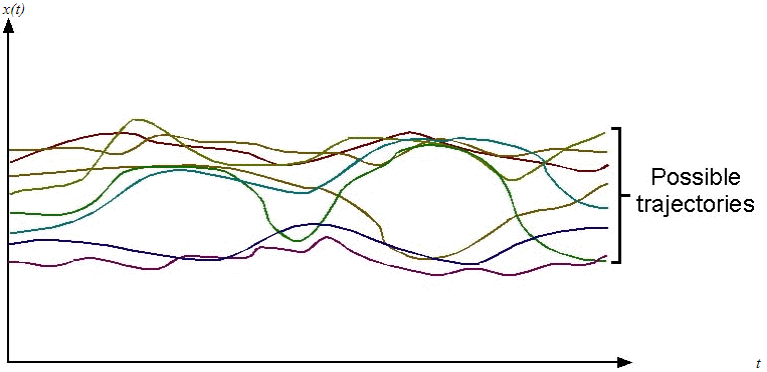
\includegraphics[width=0.47\textwidth]{figures/semantica_concreta.png}
    \caption{Rappresentazione delle possibili esecuzioni di un programma tramite curve che mostrano l'andamento dei valori in input, dello stato e dell'output in funzione del tempo.}
    \label{fig:semantica_concreta}
\end{figure}

Posti questi limiti, esistono comunque alcuni modi per affrontare il problema della verifica della proprietà di \textit{safety} che risulta essere tra quelle di maggiore interesse.
Per cercare di raggiungere tale obiettivo l'analisi dinamica considera direttamente la semantica concreta cercando di stabilire se una qualsiasi delle sue traiettorie intersechi una zona rappresentante uno stato di errore (Figura~\ref{fig:forbidden_zone}).
\begin{figure}[ht]
    \centering
    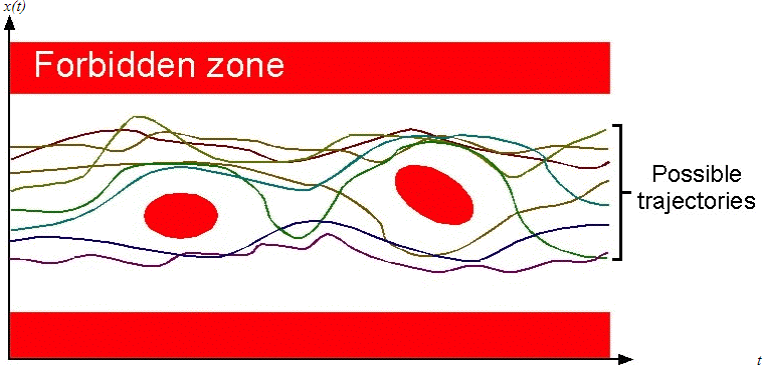
\includegraphics[width=0.47\textwidth]{figures/forbidden_zone.png}
    \caption{La \textit{forbidden zone} rappresenta gli stati in cui l'esecuzione del programma è in errore.}
    \label{fig:forbidden_zone}
\end{figure}

Tuttavia, la maggior parte delle tecniche che si concentrano sull'analisi a \textit{runtime} soffrono del problema dell'\textit{Absence of Coverage}: a causa dalla natura infinita della semantica concreta, non è possibile assicurare la proprietà di \textit{safety} perché, con questo approccio, verranno sicuramente tralasciati dei possibili flussi di esecuzione che potenzialmente potrebbero portare ad uno stato di errore.

In certi ambiti non critici questo approccio può risultare sufficiente ma, dove tale proprietà è di cruciale importanza, non è possibile lasciare spazio ad incertezze.
Perciò, la branca della verifica del software che sembra più adatta agli ambiti critici risulta essere l'analisi statica, approccio speculare rispetto a quello appena visto, che riesce ad abbassare il livello di incertezza sotto le più stringenti specifiche tramite ``\textit{approssimazione}''.

\newpage

\subsubsection{Interpretazione Astratta}
L'\textbf{Interpretazione Astratta} \cite{AbsIntNutshell} è un metodo formale dell'\\analisi statica che consiste nel considerare un sovrainsieme di tutti i possibili flussi di esecuzione di un programma (detto \textit{semantica astratta}) in modo che, se una proprietà risulta verificata per esso, lo sarà sicuramente anche per l'interezza della semantica concreta Figura~\ref{fig:semantica_astratta}.

\begin{figure}[ht]
    \centering
    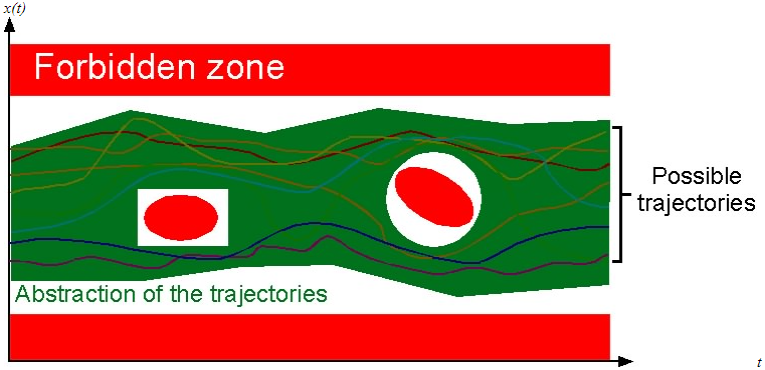
\includegraphics[width=0.47\textwidth]{figures/semantica_astratta.png}
    \caption{L'area verde rappresenta la \textit{semantica astratta}: un'approssimazione per eccesso della \textit{semantica concreta}.}
    \label{fig:semantica_astratta}
\end{figure}

I due rischi principali della definizione della semantica astratta risiedono nel processo di approssimazione.
Infatti, è possibile infrangere la proprietà di \textit{soundness} effettuando \\un'approssimazione eccessivamente restrittiva o, all'opposto, avere falsi positivi durante l'analisi a causa di un'\\approssimazione troppo ampia che interseca la zona di errore nonostante il programma non possa in alcun modo raggiungere quello stato (falso positivo).

Nonostante le limitazioni, questo approccio risulta essere effettivamente utilizzato, ad esempio  attraverso l'analizzatore statico Astrée \cite{AbsIntProfile}, da aziende come Airbus, Bosch, ESA ed altri per rispettare gli standard di sicurezza come il sopracitato DO-178C \cite{AbsIntSuccess}.
\subsection{Sottoinsiemi e sovrainsiemi di linguaggi} % MISRA
Nonostante il giovane linguaggio di programmazione \texttt{Rust} abbia convinto persino gli sviluppatori del kernel Linux \cite{RustInKernel}, ci sono state negli anni diverse proposte riguardo alla \\creazione di sotto o sovra insiemi safe di linguaggi di programmazione non memory-safe come \texttt{C} e \texttt{C++}.

\subsubsection{MISRA}
\textbf{MISRA} (Motor Industry Software Reliability Association) è un'organizzazione internazionale nata nel 1994 con \\l'obiettivo di promuovere lo sviluppo di software sicuro e affidabile, inizialmente nel settore automobilistico. Oggi, le sue linee guida e standard sono ampiamente adottati in vari settori industriali, tra cui aerospaziale, difesa, medicale e telecomunicazioni. L'organizzazione opera attraverso un processo collaborativo, coinvolgendo esperti del settore, aziende e istituzioni per sviluppare e aggiornare i suoi standard.

Questi standard forniscono regole e direttive per la scrittura di codice \texttt{C} e \texttt{C++} robusto e sicuro. Infatti, essi sono progettati per ridurre il rischio di errori nel software, migliorandone la qualità e la manutenibilità attraverso il divieto di utilizzare funzionalità del linguaggio considerate pericolose nonostante siano permesse. Le linee guida MISRA sono particolarmente utili in contesti in cui il software è soggetto a normative severe, come nei sistemi embedded o in applicazioni safety-critical \cite{MISRA}. 

Ad esempio, un programma che utilizza una variabile non precedentemente inizializzata infrange il regolamento\\ MISRA nonostante sia contemplato dallo standard \texttt{C}/\texttt{C++}.

\subsubsection{C-rusted}
\textbf{C-rusted} propone un approccio alternativo all'abbandono del linguaggio \texttt{C} verso linguaggi che offrono garanzie maggiori in termini di safety. L'idea è quella di utilizzare i concetti che si sono rivelati veramente utili in altri linguaggi, come l'\textbf{ownership} di \texttt{Rust}, e implementarli in una versione safe, secure e energy-efficient di \texttt{C}.

Questo avviene tramite annotazioni: il codice di base sarà comunque ISO \texttt{C} per mantenere la compatibilità con quanto già esistente (punto di forza caratteristico del \texttt{C}) ma il programmatore dovrà aggiungere annotazioni tramite macro (ignorate quindi dal compilatore). Esse verranno sfruttate da un analizzatore statico ad hoc che, grazie al contesto aggiunto, da esse riuscirà a garantire importanti proprietà sul codice.

Per come è stato progettato \texttt{C-rusted}, anche l'assenza di annotazioni è informativa: in ISO \texttt{C} è possibile che un puntatore qualsiasi sia \texttt{null} mentre per ottenere questo comportamento in questa versione più sicura sarà obbligatorio specificarlo tramite annotazione appunto \cite{bagnara2023crustedadvantagesrustc}.

I maggiori benefici che si hanno nel caso si scelga questa strada per scrivere codice sicuro sono:
\begin{itemize}
    \item non è necessario modificare codice già esistente se non tramite annotazioni. 
    \item non è necessario addestrare programmatori su un intero linguaggio di programmazione nuovo, ma solamente sul sistema di annotazioni.
    \item i compilatori \texttt{C} esistenti funzionano anche per \texttt{C-rusted}.
    \item i tools già esistenti per \texttt{C} funzionano anche per \texttt{C-rusted}.
\end{itemize}


\subsubsection{Safe C++}
\texttt{Safe C++}, come \texttt{C-rusted}, propone un'alternativa \\all'abbandono di un altrettanto diffuso linguaggio di programmazione a basso livello: il \texttt{C++}. Lo fa attraverso un approccio simile ma non basato su macro, ovvero quello di \textit{estendere un sottoinsieme safe} del linguaggio con meccanismi ad-hoc per implementare idee vincenti di memory safety senza l'overhead della garbage collection. Queste estensioni del linguaggio hanno richiesto l'implementazione di un compilatore \texttt{C++} (\textbf{Circle} \cite{Circle}) che supportasse i nuovi elementi della sintassi e che effettuasse i nuovi controlli statici richiesti durante la compilazione. Inoltre, si è resa necessaria una riscrittura completa (realizzata solo in parte) della libreria standard del \texttt{C++} perché ovviamente basata su codice unsafe: \texttt{Safe C++} considera unsafe tutto ciò che può portare ad \textit{undefined behavior}, come l'uso dei puntatori nel suo complesso o l'utilizzo di variabili prima della loro definizione \cite{SAFEC++}.

\subsection{Rust}
\texttt{Rust} è un linguaggio di programmazione moderno progettato per garantire sicurezza e prestazioni senza l'uso di un garbage collector. La gestione della memoria in Rust si basa su tre concetti fondamentali: \textbf{ownership}, \textbf{borrowing} e \textbf{lifetimes}. Questi meccanismi permettono di prevenire errori comuni come \textit{use-after-free}, \textit{memory leaks} e \textit{data races} in ambienti concorrenti.

\subsubsection{Ownership}

L'\textbf{ownership} è il principio cardine della gestione della memoria in \texttt{Rust}. Ogni valore ha un proprietario unico (Algoritmo~\ref{lst:ownership}) e quando il proprietario esce dallo scope, la memoria viene automaticamente deallocata.

\begin{algorithm}[ht]
    \caption{Esempio dimostrativo dell'ownership}
    \label{lst:ownership}
    \begin{lstlisting}[language=Rust, style=colouredRust]
fn main() {
    let s1 = String::from("Ciao");
    let s2 = s1; // proprieta' trasferita a s2
   
    // println!("{}", s1);  // Errore!
    println!("{}", s2);  // Stampa "Ciao"
}
\end{lstlisting}
\end{algorithm}


\subsubsection{Borrowing}

Poiché l'ownership di un valore non può essere trasferita automaticamente, \texttt{Rust} consente di prendere in prestito \\(\textbf{borrowing}) i valori attraverso le \textit{references} (\texttt{\&}) consentendo di accedere ai dati senza cambiarne il proprietario.

\texttt{Rust} distingue tra borrowing \textbf{immutabile} (Algoritmo~\ref{lst:borrowing_immutabile}) e \textbf{mutabile} (Algoritmo~\ref{lst:borrowing_mutabile}): non si possono avere più riferimenti mutabili simultanei e non ci possono essere riferimenti mutabili se ci sono già riferimenti immutabili a una stessa variabile (Algoritmo~\ref{lst:borrowing_mutabile_e_immutabile}).

\begin{algorithm}[ht]
    \caption{Esempio di borrowing immutabile}
    \label{lst:borrowing_immutabile}
    \begin{lstlisting}[language=Rust, style=colouredRust]
fn main() {
    let s1 = String::from("Ciao");
    let len = calcola_lunghezza(&s1);
    // Prestito di s1 in modo immutabile

    println!("La lunghezza di '{}' e' {}.", s1, len);
}
        
fn calcola_lunghezza(s: &String) -> usize {
    s.len()
}
\end{lstlisting}
\end{algorithm}

In questo esempio, \texttt{s1} viene prestata in modo immutabile alla funzione \texttt{calcola\_lunghezza}. Dopo la chiamata, \texttt{s1} rimane valida e può essere utilizzata.

\begin{algorithm}[ht]
    \caption{Esempio di borrowing mutabile}
    \label{lst:borrowing_mutabile}
    \begin{lstlisting}[language=Rust, style=colouredRust]
fn main() {
    let mut s1 = String::from("Ciao");
    modifica_stringa(&mut s1);  
    // Prestito di s1 in modo mutabile

    println!("{}", s1);  // Stampa "Ciao, Mondo!"
}
        
fn modifica_stringa(s: &mut String) {
    s.push_str(", Mondo!");
}
\end{lstlisting}
\end{algorithm}

Nel seguente esempio invece, \texttt{s1} viene prestata in modo mutabile alla funzione \texttt{modifica\_stringa}, che modifica la stringa aggiungendo ``, Mondo!''.
~\\
\begin{algorithm}[ht]
    \caption{Esempio di borrowing mutabile quando già immutabile}
    \label{lst:borrowing_mutabile_e_immutabile}
    \begin{lstlisting}[language=Rust, style=colouredRust]
fn main() {
    let mut s = String::from("Ciao");
        
    let r1 = &s;  // Prestito immutabile
    let r2 = &s;  // Prestito immutabile
    // let r3 = &mut s;  // Errore!
        
    println!("{}, {}", r1, r2);
}
\end{lstlisting}
\end{algorithm}


\subsubsection{Lifetimes}

I \textbf{\textit{lifetimes}} garantiscono a compile-time che le \textit{references} siano sempre valide e non puntino a memoria deallocata.

\begin{algorithm}[ht]
    \caption{Esempio gestione lifetime}
    \label{lst:lifetimes}
\begin{lstlisting}[language=Rust, style=colouredRust]
fn main() {
    let str1 = String::from("lunga stringa");
    let str2 = "xyz";
    
    let ris = longest(str1.as_str(), str2);
    println!("La stringa piu' lunga e' {}", ris);
}
    
fn longest<'a>(x: &'a str, y: &'a str) -> &'a str{
    if x.len() > y.len() {
        x
    } else {
        y
    }
}
\end{lstlisting}
\end{algorithm}

In questo esempio, la funzione \texttt{longest} restituisce il riferimento alla stringa più lunga. Il ciclo di vita \texttt{'a} garantisce che i riferimenti \texttt{x} e \texttt{y} siano validi per lo stesso periodo.

Questi concetti rendono Rust particolarmente adatto per lo sviluppo di sistemi sicuri e applicazioni ad alte prestazioni secondo le guidelines pubblicate già nel 2023 dalla CISA (Cybersecurity \& Infrastructure Security Agency), agenzia di rilevanza internazionale facente parte del dipartimento di Sicurezza Interna degli Stati Uniti \cite{CISA}.

%ownership, borrowing and lifetimes
%https://accelconf.web.cern.ch/icalepcs2019/papers/wecpr02.pdf

\section{Conclusioni}
La sicurezza e l'affidabilità del software rappresentano sfide fondamentali nel panorama tecnologico moderno, specialmente per i sistemi safety-critical. L'analisi dei principali incidenti informatici ha dimostrato come errori di programmazione, spesso legati alla gestione della memoria e della concorrenza, possano avere conseguenze devastanti. Per mitigare questi rischi, sono state sviluppate diverse strategie, tra cui linee guida per linguaggi esistenti o modifiche safe degli stessi, analizzatori statici in grado di garantire proprietà di safety, nuovi paradigmi di programmazione come quello introdotto da \texttt{Rust}. Quest'ultimo, grazie al sistema di ownership, borrowing e lifetimes, fornisce garanzie di memory safety senza la necessità di un garbage collector, rendendolo una scelta promettente per lo sviluppo efficiente di software critico. Tuttavia, l'adozione di \texttt{Rust} e di altre metodologie sicure richiede un cambiamento di mentalità e un adeguato addestramento degli sviluppatori. L'evoluzione di questi strumenti e la loro integrazione nei processi di sviluppo potrebbe ulteriormente migliorare la sicurezza del software, rendendo meno probabili gli errori umani e aumentando la resilienza dei sistemi informatici per garantire un futuro tecnologico più sicuro e affidabile.


%
% The following two commands are all you need in the
% initial runs of your .tex file to
% produce the bibliography for the citations in your paper.
\bibliographystyle{abbrv}
\bibliography{sigproc}  % sigproc.bib is the name of the Bibliography in this case
% You must have a proper ".bib" file
%  and remember to run:
% latex bibtex latex latex
% to resolve all references
%
% ACM needs 'a single self-contained file'!
%
\balancecolumns
% That's all folks!
\end{document}
